\documentclass{report}
\usepackage{graphicx}
\usepackage{hyperref}


\begin{document}

% Pagina di Copertina
\begin{titlepage}
    \centering
    \vspace*{\fill}
    \Huge \textbf{THESIS TITLE}
    \vspace{2cm} 
    
    \Large Lorenzo Ferrari

    \vspace{2cm} % Spazio aggiuntivo tra il nome e il nome dell'istituto
    
    \Large Università degli studi di Parma
    \par
    Three-year degree course in Computer Science
    
 
\end{titlepage}

%indice
\renewcommand{\contentsname}{Index}
\tableofcontents
    
    
    
    %overview 
    \chapter{overview}
    introduction and some stuff
    % Capitolo buffer overflow
    \chapter{Buffer Overflow vulnerability}
    \section{background} %---------------------fix this text ------------------
    Buffer overflow is a critical vulnerability that emerged around the 1970s and 1980s where it was 
    realized through research which leads the attacker to uncontrolled access to critical points of memory.\newline
    As the 1990s arrived the explosion of the Internet and its client-server infrastructure led large numbers of people to use buffer overflow.\newline
    Furthermore, in this period the first books were published explaining how buffer overflow works.\newline
    In the 2000s people wanted to defend themselves from these types of attacks and invented two types of mitigations:\newline
    \begin{itemize}
        \item[$\bullet$] ASLR (Address Space Layout Randomization)
        \item[$\bullet$] stack canary 
    \end{itemize}
    We will explain this mitigation later.\newline
    Between 2000s and 2010s even with the mitigations attackers managed to avoid them and still exploit buffer overflow vulnerability with technique called:\newline
        \begin{itemize}
        \item[$\bullet$] ROP (Return Oriented Programming)
        \item[$\bullet$] RET2LIBC (Return to Libc)
    \end{itemize}
    Even though vulnerability was born so many years ago it still is one of the biggest an dangerous vulnerablity.
    \clearpage
    %-----------------fix until here--------------------
    \section{How Buffer Overflow works}
    A buffer overflow occurs when the attacker can write more input than expected from the buffer, the overflow input exceeds in the memory in the location right after the buffer we are allocating, this could be very dangerous.\newline
    here's an example:
    \begin{verbatim}
    #include <iostream>
    
    int main() {
    
        char buff[30]; // buffer victim 
        printf(" insert your name: ");
        scanf("%50s",buff); 
        return 0;
    }
    \end{verbatim}
    In this example we can see a bad usage of a scanf function. In fact, this program has a char buffer with a size of 30, but the scanf function can read up to 50 chars.\newline 
    What happens if we insert more input than expected for the buffer?\newline
    State of the buffer before inserting input:
       
    \begin{figure}[h]
    \centering
    \includegraphics[width=13cm]{Organigrammi.png}
    \caption{Empty stack}
    \label{fig:example_empty_buffer}
    \end{figure}
       \clearpage
    In the example, we can notice that we have our buffer instantiated.\newline
    I wrote the question marks instead of 0x0000000000000000 because this memory at the beginning of the program is instantiated for the program we are executing, but this memory had previously been used in other contexts.\newline
    Now we will try to insert the following paylaod:
    \begin{verbatim}
        AAAAAAAAAAAAAAAAAAAAAAAAAAAAAAPPBBBBBBBBCCCCCCCC
    \end{verbatim}
    i used the "A" to fill the buffer "P" for the remaining buffer before RBP, "B" for overwriting the saved base pointer,
    C for overwriting the return address.
    this will cause a buffer overflow because when we get to the assembly instruction leave and ret it will not find the instruction 0x4343434343434343 and the program will receive a segmentation fault.
    \begin{figure}[h]
        \centering
        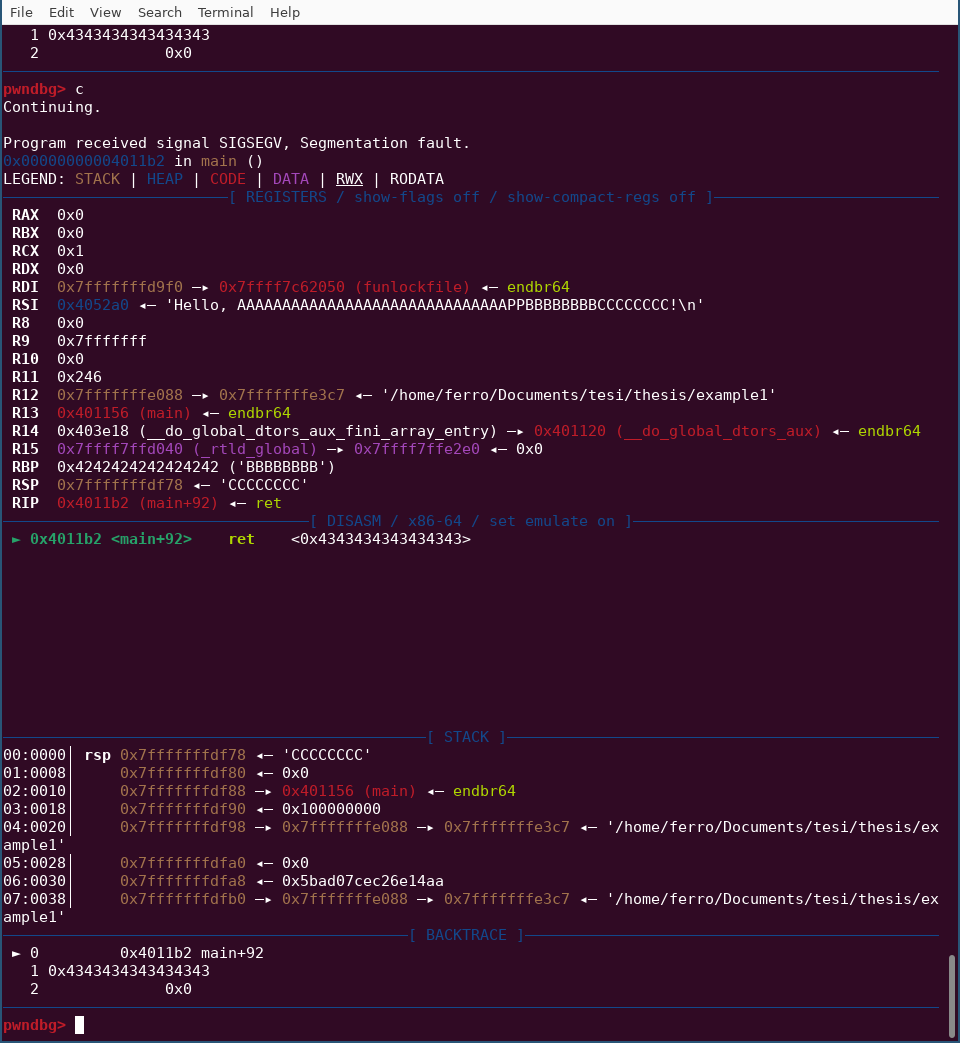
\includegraphics[width=0.9\linewidth]{example1.png}
        \caption{buffer overflow triggered}
        \label{fig:empty stack}
    \end{figure}
    \newpage
    
    This is how looks the stack after sending this payload:
    \begin{figure}
        \centering
        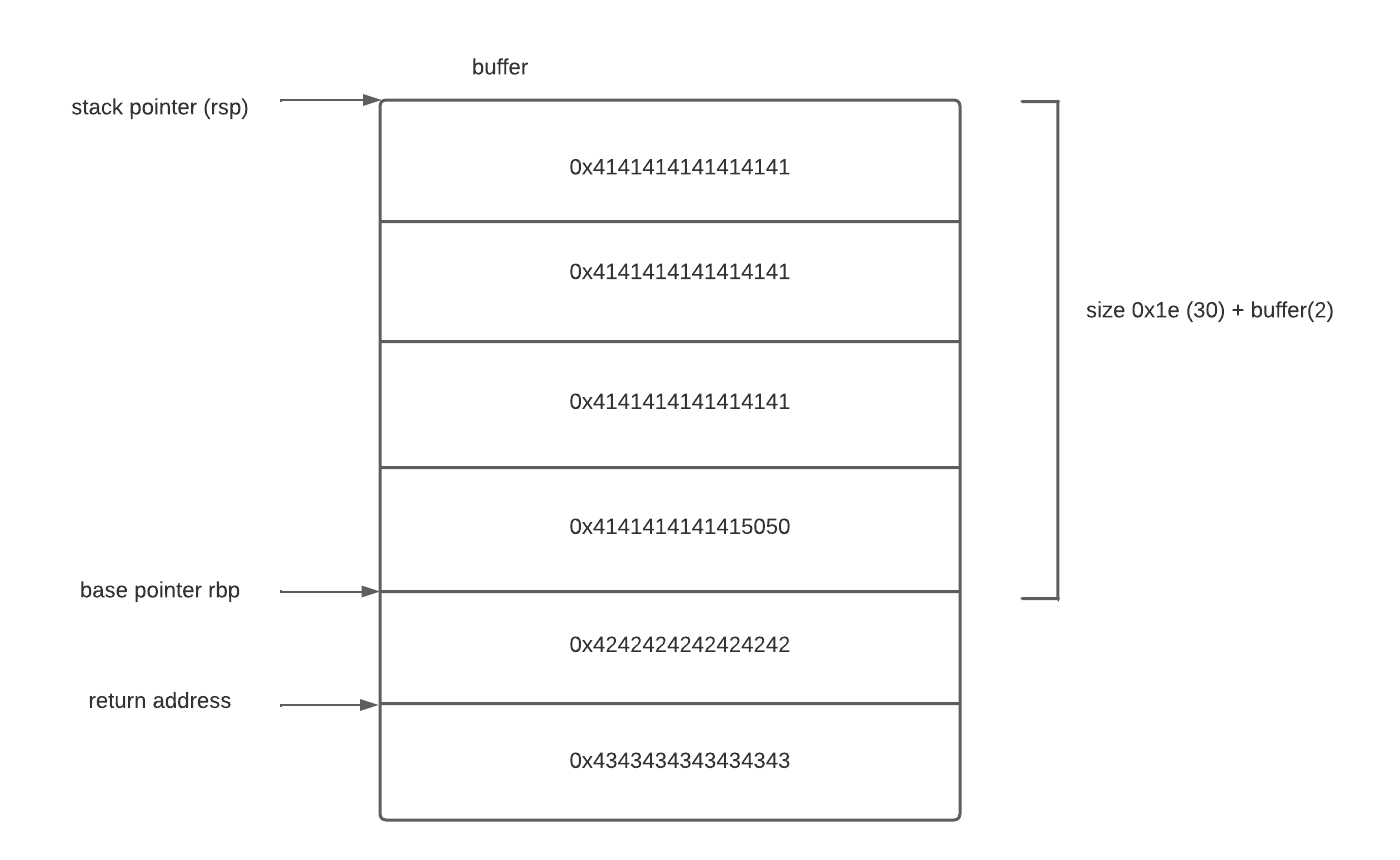
\includegraphics[width=1\linewidth]{stack_after_overflow.png}
        \caption{Stack after the overflow}
        \label{fig:stack w overflow}
    \end{figure}
    \clearpage
    \chapter{Mitigations against Buffer Overflow}
    \section{Stack Canary}
    The stack canary is a protection that was invented in the 90s to prevent a buffer overflow from occurring.
    It consists of generating a protection value, generated at run time and therefore different for each time a program is executed, but remains for the entire execution of the program.
    The stack canary is placed before important metadata such as the saved base pointer and return address.
    Before executing the epilogue of the function, the integrity of the value of the stack canary is checked. If this has been modified or tampered with, the program will end immediately with the following exit code:
    \begin{verbatim}
    *** stack smashing detected ***: terminated
    \end{verbatim}
    Compilers like gcc by default compile with stack canary, by analyzing the decompiled file the compiler will insert the following lines of code to insert the stack canary.\newline
    \begin{verbatim}
    if (local_10 != *(long *)(in_FS_OFFSET + 0x28)) {
                    /* WARNING: Subroutine does not return */
    __stack_chk_fail();
  }
    \end{verbatim}
    
    The name derives from a small historical note. In fact, the name "stack canary" was inspired by the technique used in coal mines.\newline
    To avoid entering an area of the mine with high levels of toxic gases, they would let a canary fly ahead. If the canary died, passage was prohibited; otherwise, they could pass.
    \clearpage
    Following is the photo of the stack extracted from GDB. As we can see, I inserted two commands:
    \begin{itemize}
      \item \hspace{1em} canary: This command shows the possible canaries of this code.
      \item \hspace{1em} stack 20: This command shows 20 stack instances.
    \end{itemize}
    As we can see, at address 0x7fffffffdf68, we have the value 0xe1509a30995e5f00, which is our stack canary.
    \begin{figure}
        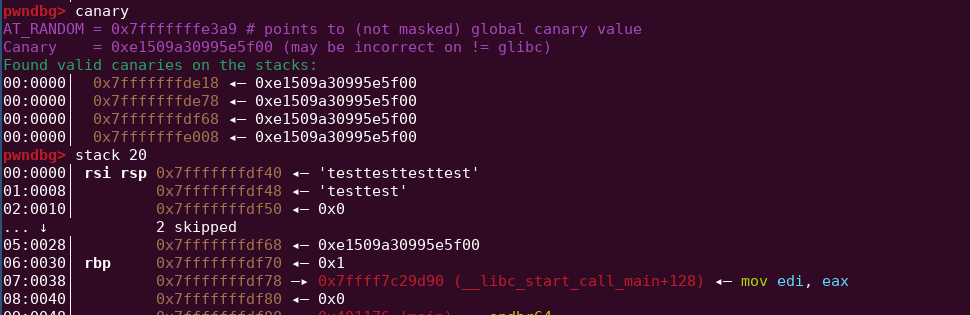
\includegraphics[width=1.3\linewidth]{photo_of_the_stack_with_canary.png}
        \caption{ stack canary on gdb }
        \label{fig:  photo stack canary}
    \end{figure}
    \clearpage
    \section{ASLR}
    ASLR stands for Address Space Layout Randomization and is a technique they invented to protect operating systems from memory attacks.\newline
    In fact ASLR has the task of randomizing sections of memory such as heap stacks and shared libraries every time a program or operating system is launched.\newline
    ASLR with the stack canary seen previously and PIE that we will see later are mitigations mainly developed to avoid buffer overflow, in fact ASLR for example avoids us from jumping into memory locations that would be in fixed positions if it were not for this mitigation, and it avoids many attacks.\newline
    \begin{figure}[h]
        \centering
        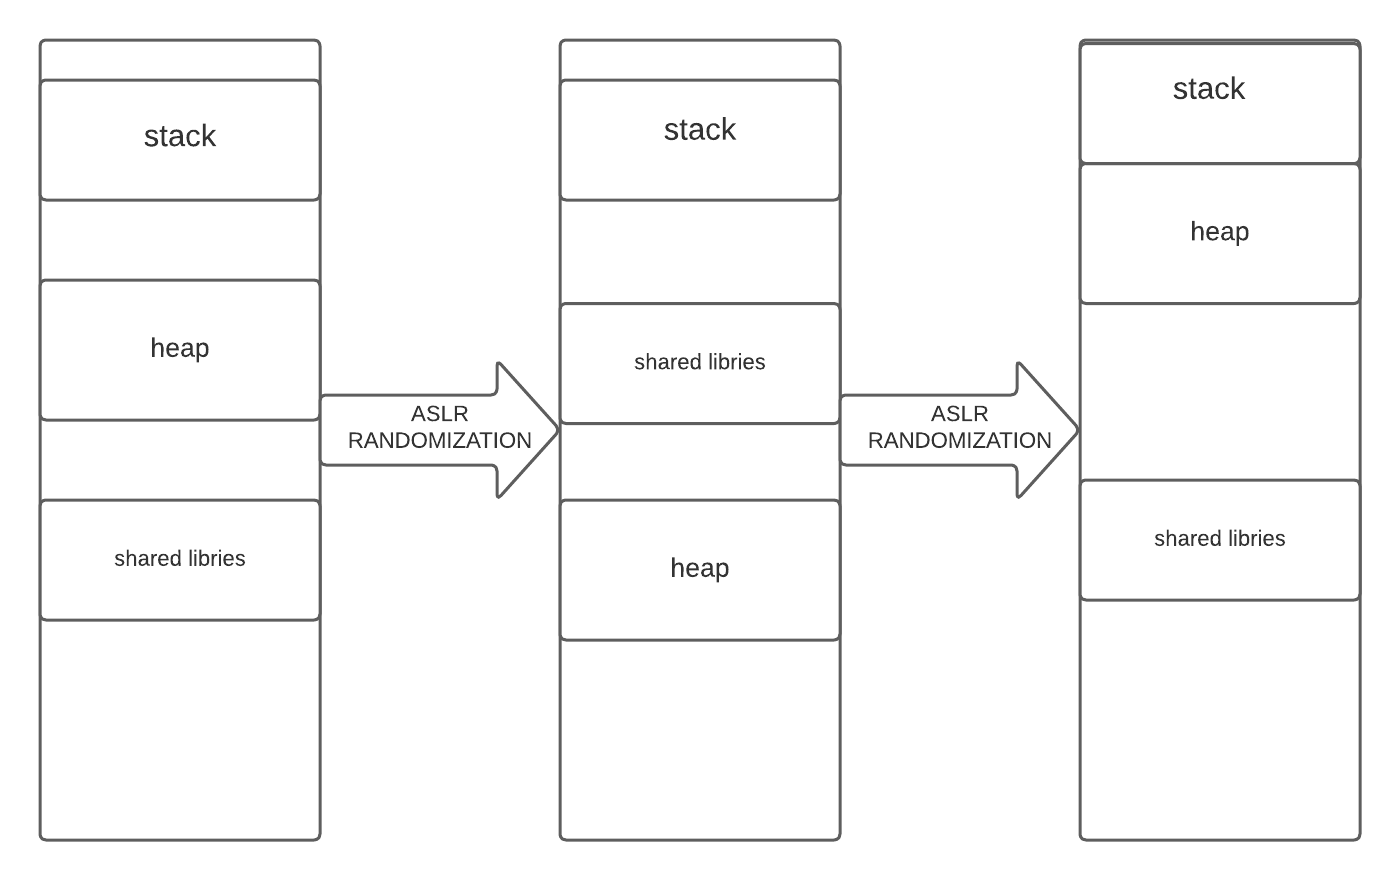
\includegraphics[width=1\linewidth]{ASLR_stack_image.png}
        \caption{memory with aslr }
        \label{fig:enter-label}
    \end{figure}
    \clearpage
    \section{PIE}
    PIE stands for Position Independent Executable and is very similar to ASLR, in fact it follows the same concept as ASLR but with the binary assembly memory region.\newline
    As can be interpreted from the name Position Independent gives the possibility for a binary to be loaded and executed in memory at arbitrary addresses, this means that the program data instead of referring to addresses in fixed memory are referenced through the use of an offset random to the current position where it is loaded plus the offset.\newline
        \begin{tabular}{|c|c|c|c|}
      \hline
      ASLR  & PIE & Binary Address & Libc Address \\
      \hline
      disable & disable  & 0x400000 & 0x7ffff7d86000 \\
      disable & disable  & 0x400000 & 0x7ffff7d86000\\
      disable & activated   & 0×555555554000 & 0x7ffff7d86000 \\
      disable & activated   & 0×555555554000 & 0x7ffff7d86000 \\
      activated  & disable  &  0x400000 & 0x7fe7833eb000 \\
      activated  & disable  &  0x400000& 0x7f1a44191000 \\
      activated  & activated   & 0×555555554000 & 0x7f29d6ebd000 \\
      activated  & activated   & 0×555555554000 & 0x7f7d008a0000 \\
      \hline
    \end{tabular}
    \clearpage
    \section{Buffer Overflow attack and mitigations bypass}
    to be continued
    \clearpage
    \section{explanation of a challange and exploit analyses}
    to be continued
    
    
    %capitolo heap overflow 
    \chapter{Heap Overflow Vulnerability}
    \section{How it works a Heap Overflow}
    to be continued
    \clearpage
    \section{overview challenge and attack planning}
    to be continued
    \clearpage
    \section{exploit analisys}
    to be continued
    \clearpage
    %capitolo double free
    \chapter{Double Free Vulnerability}
    \section{How it works a Double Free}
    to be continued    
    \clearpage
    \section{overview challenge and attack planning}
    to be continued
    \clearpage
    \section{exploit analisys}
    to be continued
    \clearpage
    % capitolo conclusioni
    \chapter{Conclusion}
    to be continued
    \section{online references}
    \href{https://it.wikipedia.org/wiki/Home_page}{.....}
    \clearpage
\end{document}
